\documentclass[12pt,a4paper,titlepage]{article}

\usepackage{times}
\usepackage{setspace}
\usepackage{textcomp}
\usepackage[a4paper,left=1in,top=1in,right=1in,bottom=1in]{geometry}

\usepackage[english]{babel}
\usepackage[backend=biber]{biblatex}
\usepackage{csquotes}

\usepackage[bookmarks]{hyperref}
\hypersetup{colorlinks=true,allcolors=black}
\usepackage{hypcap}
\usepackage{graphicx}
\usepackage{caption}
\usepackage{subcaption}
\usepackage[section]{placeins}

\bibliography{sources.bib}


\doublespacing{}
\oddsidemargin = 0pt
\headheight = 0pt
\topmargin = 0pt
\headsep = 0pt
\marginparwidth = 0pt
\textwidth = 450pt


\begin{document}

\title{IIR IP}
\author{Kevin Bloom \\ Rev A}
\maketitle

\newpage

\tableofcontents

\newpage

\section{Introduction}
When selecting this project, I was under the assumption that it would be fairly
easy to complete; seeing as completing this task in software isn't a huge
deal. To my surprise, this was far from true. The calculation for IIR is quite
difficult to complete in hardware, as I will discuss in this report. I will be
discussing the theory behind the IIR in hardware, the major issues that can
occur, and how one could complete this task in the future.

\subsection{Important Files}
Inside of this project, there are a few different files that are important.
Firstly, my notebook. This file is entitled \texttt{notebook.org} and contains
information on my process throughout the semester. You can open it with a text
editor of choice, or you can view the exported \texttt{notebook.html}
file. Please note that the HTML version doesn't contain all of the clock
stamps. Inside of \texttt{presentation/} is the presentation and its source. The
source for this report can be found in \texttt{report/}. Inside of
\texttt{projects/} will be all of the different projects that I worked on. The
important ones to note are: \texttt{2nd-order-single-section/},
\texttt{complex-iir/}, and \texttt{the-really-big-one/}.

Just so that it's easier to find your way, I will do a quick description of each
project. This will prevent you from having to search
around. \texttt{2nd-order-single-section/} is a design that only uses a single
section BiQuad. This was used to prove that there was something wrong with the
BiQuad implementation of the IP. \texttt{complex-iir/} contains a design that
doesn't use the Zynq. It does everything in hardware. The current setup uses
internally selected coefficients, opposed to the normally externally fed
coefficients. Lastly, \texttt{the-really-big-one/} is a design that uses pretty
much everything. It is set up with 4 BiQuads cascaded serially and uses the dmux
and mux IPs to make the design generic.

\subsection{Licensing}
The last thing that should be noted is that any code that was written by me,
Kevin Bloom, is licensed under the GNU Lesser General Public License (LGPL)
version 3 or above. A copy of this license is found in the \texttt{LICENSE} file
in the root directory of the project. This includes any IIR, FIR, mux, and demux
VHDL files and any IIR communication C files. It is important that whomever is
given the projects is also given the \emph{same freedoms as me, Kevin
  Bloom}. Please make sure that this happens. Also, if someone is given this
project \emph{without those freedoms}, please
\underline{\href{https://github.com/nuclearkev/iir-hardware}{my GitHub page}} to
receive copies of my code \emph{with those freedoms}.


\section{Single-Section}
This section I will discuss the problem related to using a single-section or
standard form IIR in hardware. The term \emph{single-section} is referring to
the number of sections, or stages, needed to complete the calculation. In a
single-section filter, there is only 1 section needed. This means that there is
no need for cascading multiple stages together. You can convert your IIR filter
to a single-section in MATLAB by selecting the \texttt{Convert to Single
  Section} under the \texttt{Edit} tab.

\subsection{Coefficients}
As soon as you convert your filter to a single-section, you will immediately
notice that there isn't a gain listed. This is most likely because the gain is
incorporated into the coefficients already and is not something you should be
concerned about. Another thing you may notice is that the number of coefficients
in each pair (whether numerator or denominator) is probably larger than in the
multi-section or \emph{BiQuad} form. In a BiQuad form both coefficient arrays
have 3 elements yet in the single-section they may have more. Take a look at the
follow example in \textbf{Figure 1}:

\begin{figure}[!htb]
  \centering
  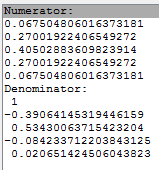
\includegraphics[height=5cm]
                  {../presentation/standard-coeffs-48kfs-10800fc.png}
                  \caption{$F_s = 48$kHz, $F_c = 10.8$kHz}
\end{figure}

Here, you will see that we have 5 coefficients in each array. This may not seem
problematic and it really isn't. It would be fairly easy to design hardware that
could take a varying number of coefficients. All you would need to do have a
maximum number of coefficients set, then depending on the number passed in, you
would clear the not-in-use registers to zero. In theory, this would work
great. However, there is still a major issue with using single-section that
doesn't have to do with number of coefficients. It has to do with the
\emph{size} of the coefficients. Take a look at \textbf{Figure 2} and you will
notice 2 interesting things: the numerator coefficients are quite small and the
denominator coefficients are big.\footnote{In perspective to the numerator
  coefficients}

\begin{figure}[!htb]
  \centering
  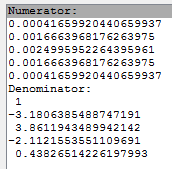
\includegraphics[height=5cm]
                  {../presentation/standard-coeffs-100kfs-5kfc.png}
                  \caption{$F_s = 100$kHz, $F_c = 5$kHz}
\end{figure}

So, what's the big deal? Well, if you attempt to convert those numbers to fixed
point uses our standard quantisation 1.15\footnote{This is fancy for, 1 bit
  integer and 15 bits fractional. We could just as easily have said quantisation
  2.14; 2 bits integer and 14 bits fractional.} you get overloaded values in the
denominator and zeros in the numerator. That being said, we can generalize this
problem by saying that the the numerator coefficients approach zero and the
denominator coefficients approach infinity. Due to this problem, it is nearly
impossible to create a generic IIR filter using the single-section
method.\footnote{Well, one that's worth a damn that is.}

\subsection{Benefits}
Just because single-section isn't the best way to do things, it still have some
benefits over the BiQuad method. Firstly, it is far simpler. You don't need to
mess around with extra signals and cascading. It makes the design, as a whole,
much simpler. Secondly, it requires less hardware. This is a good thing,
especially if you are on limited hardware such as the Lattice ICE family of
FGPAs. If you have a specific application in which the cutoff isn't going to
change and you can pick the sample frequency, this may be the better
route. For this project, it is \emph{not} sufficient, thus, we need to
investigate another method.

\newpage

\section{BiQuad}
BiQuads are simple 2nd order filters that can be cascaded together to complete
larger order applications. The BiQuad solves the biggest problem found with the
single-section design, namely coefficient size. Don't get too excited because it
opens up a new can of worms. Granted, these problems are far easier to handle,
thus, making the BiQuad a far better way to execute IIRs in hardware. Let's
break down the BiQuad just as we did the single-section.

\subsection{Coefficients}
As mentioned, the BiQuad is a 2nd order filter when we look at it
atomically. There 2nd order filters get cascaded together, whether in serial or
parallel, to complete filters of higher order. That being said, the number of
coefficients found in each stage remains the same. This is extremely beneficial
in the generic case because we no longer have to modify the IP or internal
design of the IIR to change the number of coefficients.\footnote{Only if we
  went outside of out preset limits, obviously.} If we wish to increase the
order of the system, we can simply add in the necessary stages. \textbf{Figure
  3} is an example of a 4th order filter set of coefficients in BiQuad form.

\begin{figure}[!htb]
  \centering
  \begin{subfigure}[b]{0.3\textwidth}
    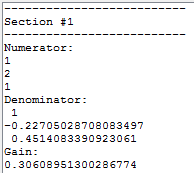
\includegraphics[width=\textwidth]
                    {../presentation/biquad-coeffs-section1-48kfs-10800fc.png}
  \end{subfigure}
  \begin{subfigure}[b]{0.3\textwidth}
    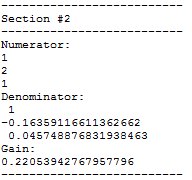
\includegraphics[width=\textwidth]
                    {../presentation/biquad-coeffs-section2-48kfs-10800fc.png}
  \end{subfigure}
  \caption{$F_s = 48$kHz, $F_c = 10.8$kHz}
\end{figure}

\begin{figure}[!htb]
  \centering
  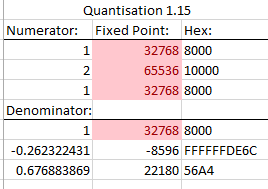
\includegraphics[height=5cm]
                  {../presentation/overflow-coeffs.png}
                  \caption{Overflowed Coefficients}
\end{figure}

\newpage

So, there we have it. The solution to everything. Coefficients look fine, we are
done, right? Wrong. These coefficients have 1 major flaw still: they
overflow. The numerator coefficients overflow when using our standard
quantisation 1.15, therefore, we need to \emph{scale} these
coefficients. Scaling will give us coefficients that we can easily convert to
fixed point with no issues. Then all we much do is multiply by some gain at the
end to get the proper outputs. If you don't believe me about them overflowing,
look at \textbf{Figure 4}. In that figure we the coefficients, their fixed point
value, and that value in hex. You will notice that 1 and 2 \emph{both}
overflow.\footnote{1 overflows because the sign bit is high, and 1 is not
  negative.}

\subsection{Scaling}
Thanks to MATLAB, scaling is quite easy to do. All you must do is go into the
\texttt{Edit} drop down menu, and select \texttt{Reorder and Scale Second-Order
  Sections ...} and you will see the dialog shown in \textbf{Figure 5}.

When you first open the window, the \texttt{scale} check box will be
unchecked. Check it. You now have access to a few different scaling options. I
recommend that you use the \emph{L2} method. This is because it seems to
diminish the coefficients very well yet doesn't have a huge gain at the end. The
gain seems to be close to 1 for the most part. This is nice because you don't
have to worry about adding in gain multipliers, since they are a waste of
hardware and time. I also recommend that you keep \texttt{Maximum Numerator} and
\texttt{Numerator Constraint} at the default. \texttt{Overflow Mode} should be
set to \emph{Saturate}, \texttt{Scale Value Constraint} to \emph{Powers of Two},
and \texttt{Max Scale Value} to \emph{16}. Then \emph{apply} the changes.

Once the changes have been applied, you should see something similar to
\textbf{Figure 6}. Your numerator coefficients should smaller and your gains
should have changed to some fraction of denominator that is a power of
two.\footnote{Sometimes they won't be exact.} In the figure, I show that the
values do not overflow anymore. I also show the big gains at the end. As noted
earlier, the L2 scaled coefficients are slightly larger and but have a smaller
gain at the end. It's close enough to 1, so you could get away with ignoring
it altogether.

\begin{figure}[!htb]
  \centering
  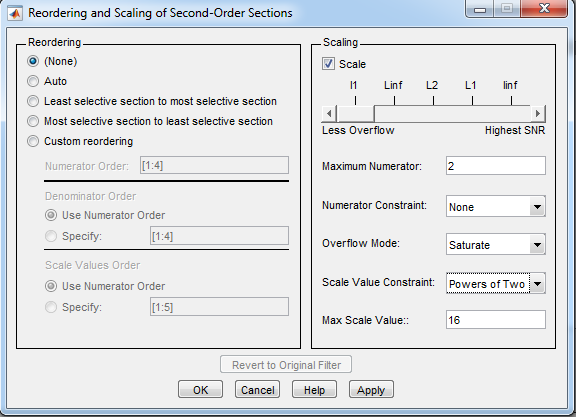
\includegraphics[height=8cm]
                  {../presentation/scaled-window.png}
                  \caption{Scaling Window}
\end{figure}

\begin{figure}[!htb]
  \centering
  \begin{subfigure}[b]{0.4\textwidth}
    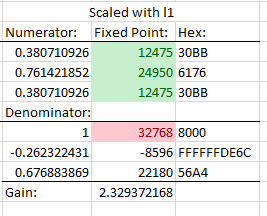
\includegraphics[width=\textwidth]
                    {../presentation/scaled-with-l1.png}
  \end{subfigure}
  \begin{subfigure}[b]{0.4\textwidth}
    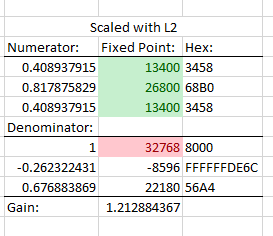
\includegraphics[width=\textwidth]
                    {../presentation/scaled-with-L2.png}
  \end{subfigure}
  \caption{Scaled Coefficients}
\end{figure}

\subsection{Benefits}
As we already discussed, the BiQuad is much better than the single-section; but
what are some of the major benefits to using it. Firstly, the size of the
coefficients are controllable. This allows use to have the opportunity to run
any filter we want. Secondly, BiQuads can be made generic. With a little added
work, you can create a BiQuad design that is generic enough that you can change
the order of the filter, without having to modify the number of stages. All you
need is a demux at the end. This demux would select which output you wish to
take from. For example, you have a design that has 4 stages (8th order) but you
wish to implement a 6th order filter. You don't need to remove that last stage
if you have a output selecting demux. You can give coefficients to the first 3
stages and then select the output to come from stage 3, and there you have it!
This is extremely handy because it allows us to very easily change the order of
the filter without having to mess around with much. I believe that these are the
2 biggest benefits to using the BiQuad method.

\section{IIR IP}
Now that we have most of the major theory out of the way, we can start to
discuss the actual IP. I'm just going to go right down the line on this one,
skipping over the coefficients input process (see \hyperref[sec:zynq]{Zynq
  Communication} for that). First and foremost, the IP's exterior layout is
  down in \textbf{Figure 7} below.

\begin{figure}[!htb]
  \centering
  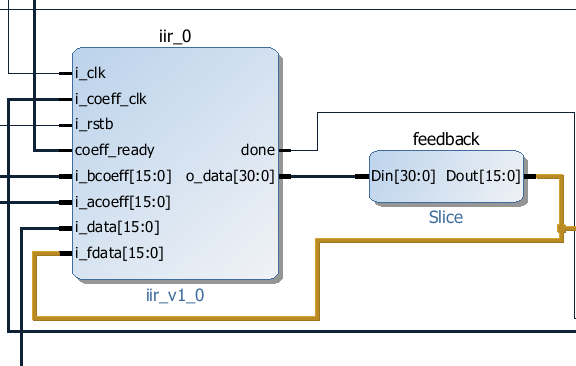
\includegraphics[height=6cm]
                  {../presentation/iir-ip-external-feedback.png}
                  \caption{IIR IP in Block Format}
\end{figure}

Let me explain what each input is and its function. Starting at the top,
\texttt{i\_clk} is the clock for the system. This is hooked directly to the
either the sample clock or the end-of-conversion signal from the
XADC. \texttt{i\_coeff\_clk} is the clock for shipping in the coefficients from
the Zynq. \texttt{i\_rstb} is the rest for the IP; it is hooked to the system
reset. \texttt{coeff\_ready} is the signal that tells the IP that the Zynq is
ready to ship it new coefficients. Think of it as a start signal for the Zynq
communication. \texttt{i\_bcoeff} and \texttt{i\_acoeff} are the coefficients
input signals that are 16 bits width. These are hooked directly to the GPIO that
controls that stage. \texttt{i\_data} is the data from the XADC. I use DRP, so
this is taken from the \texttt{do\_out} signal of the XADC in DRP
mode. \texttt{i\_fdata} is the feedback data. \texttt{done} is the done
signal. This is used to start the DA2. Lastly, we have \texttt{o\_data}, which
is the output data. Note that this is of width 31 bits. Due to Vivado
limitations on IP creation, it wouldn't let me go past 100 in/out bits. I have
exactly 100 with \texttt{o\_data} at 31 bits.

Let us now look inside the IP and see how it works. Due to the number of images,
they were put into an appendix. Please see Appendix A: Inside the IP for the
screenshots I refer to here. The first thing the IP does (besides getting
coefficients) is inputting data. As seen in \textbf{Figure \ref{fig:a0}}, the
feedforward and feedback data is pulled directly from the input signals and
is anded with there respective internal array. This fancy operation found on
lines 78 and 79 are the hardware engineer's quick and dirty way of shifting
elements in an array. This pushes the data from indexes 0-2 to 1-3 then shoves
the anded value into index 0. Keep in mind that both array are the \emph{same
  size}. This is for symmetry in the design. Normally the feedback array would
only need 3 values, however, this throws off the design's symmetry and makes it
look bad.

The next 4 processes I will discuss in a single paragraph because they are all
related very closely. They are found in \textbf{Figures \ref{fig:a1} to
  \ref{fig:a4}}. These are the arithmetic processes; they do the actual IIR
calculation. However, in hardware it is a good idea to follow the rules of
\emph{pipelining} when doing calculations. Pipelining allows for higher clock
frequencies, reduces synthesis times, and increases throughput for the
system. For those reasons, I pipelined the entire design. In \textbf{Figure
  \ref{fig:a1}}, you will see the multiplication. Notice that it's in a for loop
and stores each multiplication into a new register in the respective array. Also
note that on the final loop, when $k = 2$, the multiplication for the feedback
will always be zero. In the next process, \textbf{Figure \ref{fig:a2}}, we start
the additions. Notice that I must resize the registers before the addition. Both
of the first stage addition arrays are 1 bit wider than the multiplication
arrays. This will protect us against the overflow that may occur. The same thing
is completed in the final addition stage, \textbf{Figure \ref{fig:a3}}. Finally,
we subtract the feedforward data by the feedback data in \textbf{Figure
  \ref{fig:a4}}.

The final process in the design is the data output process found in
\textbf{Figure \ref{fig:a5}}. This one simply sets the \texttt{done} signal high
and outputs the data. Notice that I use cast the \texttt{r\_final\_sum} register
into an \texttt{std\_logic\_vector} because all the arithmetic is done in
\emph{signed} and you cannot output a signed value.

\section{Zynq Communication}
\label{sec:zynq}
The last piece of the puzzle is how the Zynq gets incorporated into the
system. This is fairly simple because all it does is use GPIOs and a clock! Once
again, due to the large number of images, they are found in Appendix B:
Communication Protocol. In \textbf{Figure \ref{fig:b0}}, you will see how the
GPIOs hook up in the block design. There isn't really anything special about
this, so there isn't much to say. Next in the queue is \textbf{Figure
  \ref{fig:b1}}, which is the process within the IIR IP that handles the
coefficient accepting. Notice that it uses the \texttt{coeff\_ready} signal to
reset the coefficient registers and the looping variable. It then uses the
rising edge of \texttt{i\_coeff\_clk} to say when to grab the next
value. Lastly, \textbf{Figure \ref{fig:b2}} shows the code from the Zynq which
is very simple. The arrays, \texttt{b\_coeff} and \texttt{a\_coeff}, contain the
coefficient that you wish to upload to the IP. Earlier in the program, the
\texttt{coeff\_ready} signal was set high. Then, within this loop the
\texttt{i\_coeff\_clk} signal is toggled and the GPIO values are changed. This
is how simple the communication is.

\section{Example Outputs}
Found in Appendix C: Examples will be some example outputs of the system
discussed in this report. In \textbf{Figure \ref{fig:c0}}, you will see the
attempt at a lowpass filter. First thing you'll probably notice is that the
amplitude is off. We are about 30dB too low. Other than that, this filter
actually preforms as intended. It is dead at around 10kHz, which is what it
should be. The next example isn't as good, as shown in \textbf{Figure
  \ref{fig:c1}}. This time the first thing that you will notice is that the
passing section is very unstable. However, it does ``pass'' the correct
frequencies. Although it isn't pretty, it still works to an extent. The final
example, shown in \textbf{Figure \ref{fig:c2}}, is a complete mess. It is an
attempt at a bandpass and, as you will see, isn't a very good one. It has a
passing region but it's very unstable and isn't the correct frequency
range. It's off by about 3kHz. In the end, these examples are not great but do
so that the system \emph{works} just very poorly.

\section{Conclusion}
In the end, the project fell flat and didn't work as intended. This isn't,
however, a bad thing. Along with the struggles of the project, I learn a lot
about IIRs and hardware design in general. This information may be useful later
in my career. There are many reasons as to why the project didn't work. Some of
the problems may have been the following: Not multiplying by the gain, no FSM in
the IP, and not accurate data/coefficient. Not multiplying by the gain could be
the reason the amplitude was so low. However, I don't believe this is entirely
what caused the problem due to the fact all the gains where close to 1
(somewhere between .8 and 1.3). Even if we multiplied by these gains, it would
only vary the amplitude slightly. Not having a FSM in the IP could be one of the
things that caused it's inconsistency. Without an FSM, we don't have a way to
flow control the process. Instead, I rely on sensitivity lists to move to the
next process. It would have probably been a better idea to use that, but with an
FSM that would only allow certain things to happen once a blocker register was
set or reset. Lastly, there is a surprising amount of inaccuracy in using 16 bit
coefficients. Some of the more high quality designs I saw online used 32 bit
coefficients. This may or may not have had something to do with the
inconsistency of the output.

When it comes down to it, the IIR is not something that is favorable to do
hardware. There are a lot of areas that can cause issues due to the complex
nature of the calculation. Just the arithmetic itself is difficult in hardware
because of overflowing and scaling. On top of this, attempting to make it
generic is something that seems reasonable but may not be easily
completed. Because of all the issues and complexities of the IIR, I believe that
this is an application for a microcontroller or processor. On those systems, we
don't have \emph{any} of these issues. We can use floats or doubles for all the
data, eliminating all the overflow, scaling, and coefficients related
problems. In conclusion, I believe that the IIR is \emph{not} a good application
for a FPGA but an application for a microcontroller instead.

\newpage

\appendix

\section{Inside the IP}
\begin{figure}[!htb]
  \centering
  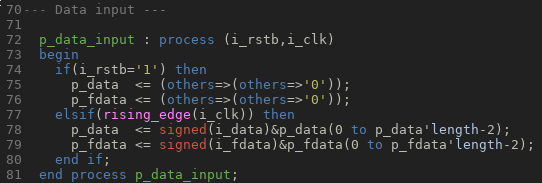
\includegraphics[width=\textwidth]
                  {../presentation/data-input.png}
                  \caption{Data Input Process}
                  \label{fig:a0}
\end{figure}
\begin{figure}[!htb]
  \centering
  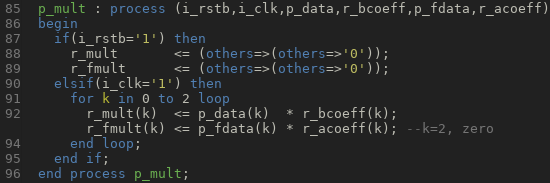
\includegraphics[width=\textwidth]
                  {../presentation/mult.png}
                  \caption{Multiplication Process}
                  \label{fig:a1}
\end{figure}
\begin{figure}[!htb]
  \centering
  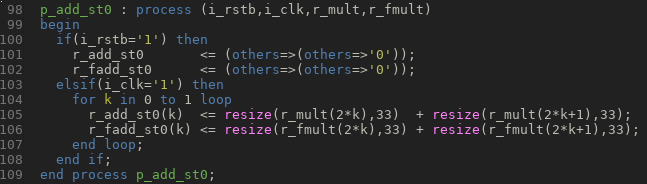
\includegraphics[width=\textwidth]
                  {../presentation/add0.png}
                  \caption{First Addition Process}
                  \label{fig:a2}
\end{figure}
\begin{figure}[!htb]
  \centering
  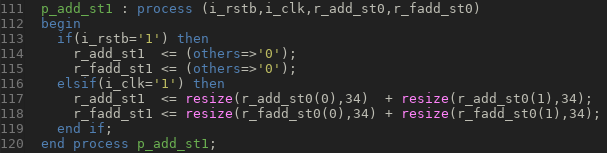
\includegraphics[width=\textwidth]
                  {../presentation/add1.png}
                  \caption{Second Addition Process}
                  \label{fig:a3}
\end{figure}
\begin{figure}[!htb]
  \centering
  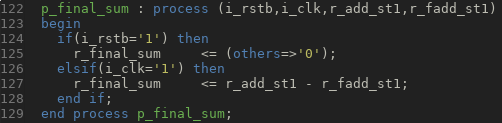
\includegraphics[width=\textwidth]
                  {../presentation/final-add.png}
                  \caption{Feedfoward Feedback Subtraction Process}
                  \label{fig:a4}
\end{figure}
\begin{figure}[!htb]
  \centering
  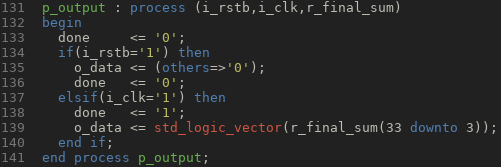
\includegraphics[width=\textwidth]
                  {../presentation/output.png}
                  \caption{Data Output Process}
                  \label{fig:a5}
\end{figure}


\newpage

\section{Communication Protocol}
\begin{figure}[!htb]
  \centering
  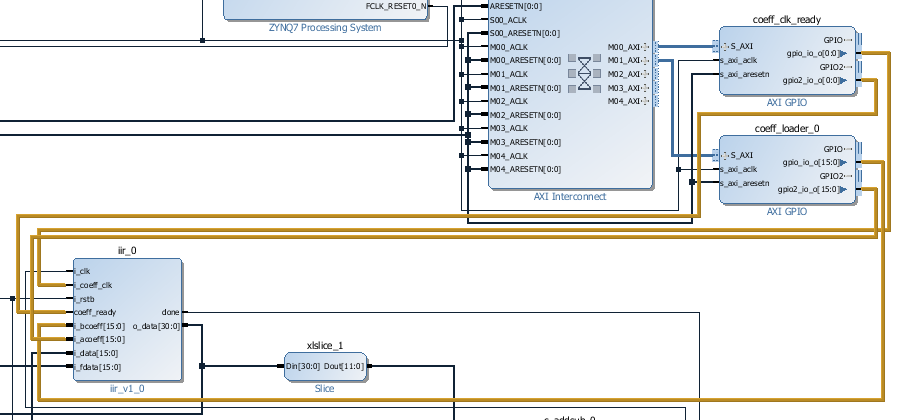
\includegraphics[width=\textwidth]
                  {../presentation/zynq-communication-design.png}
                  \caption{GPIO Hook Ups}
                  \label{fig:b0}
\end{figure}
\begin{figure}[!htb]
  \centering
  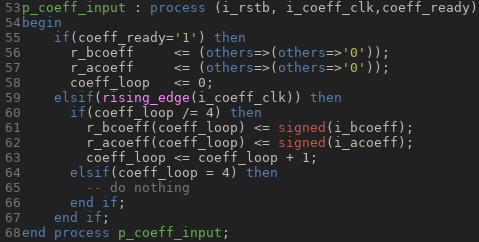
\includegraphics[width=\textwidth]
                  {../presentation/coeff.png}
                  \caption{Coefficient Input Process}
                  \label{fig:b1}
\end{figure}
\begin{figure}[!htb]
  \centering
  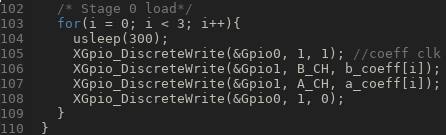
\includegraphics[width=\textwidth]
                  {../presentation/zynq-coeff.png}
                  \caption{Coefficient Output Loop}
                  \label{fig:b2}
\end{figure}

\newpage

\section{Examples}
\begin{figure}[!htb]
  \centering
  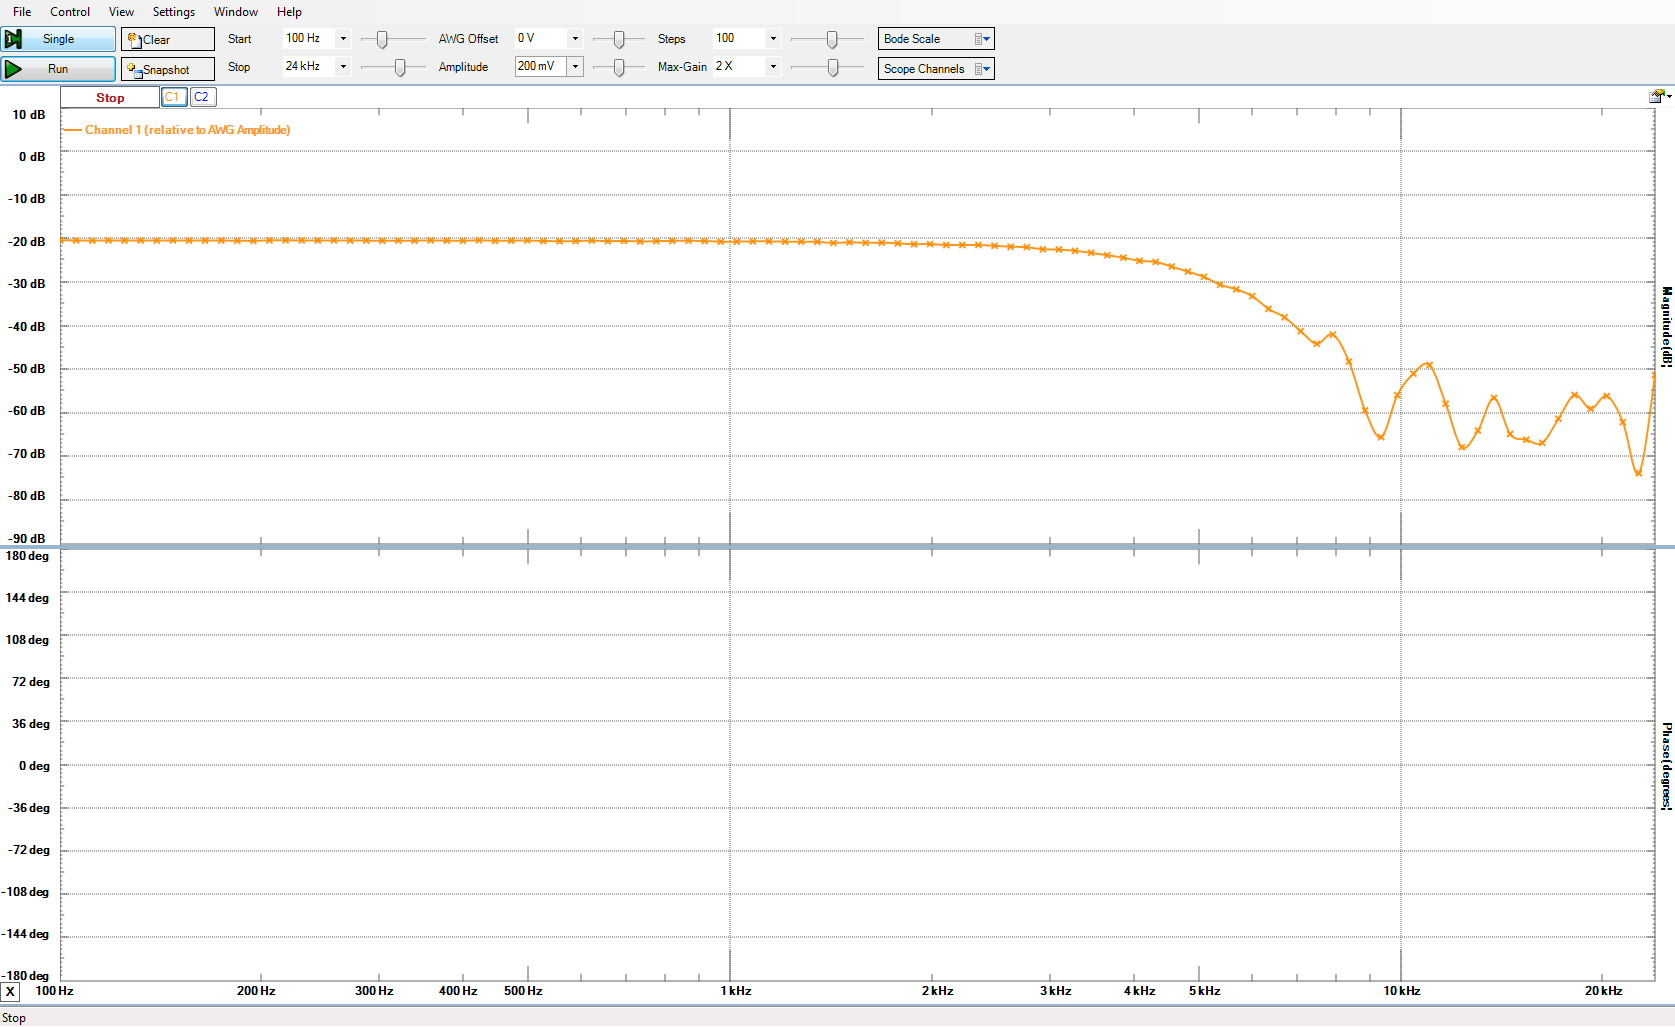
\includegraphics[width=\textwidth]
                  {../presentation/lowpass-final.png}
                  \caption{GPIO Hook Ups}
                  \label{fig:c0}
\end{figure}
\begin{figure}[!htb]
  \centering
  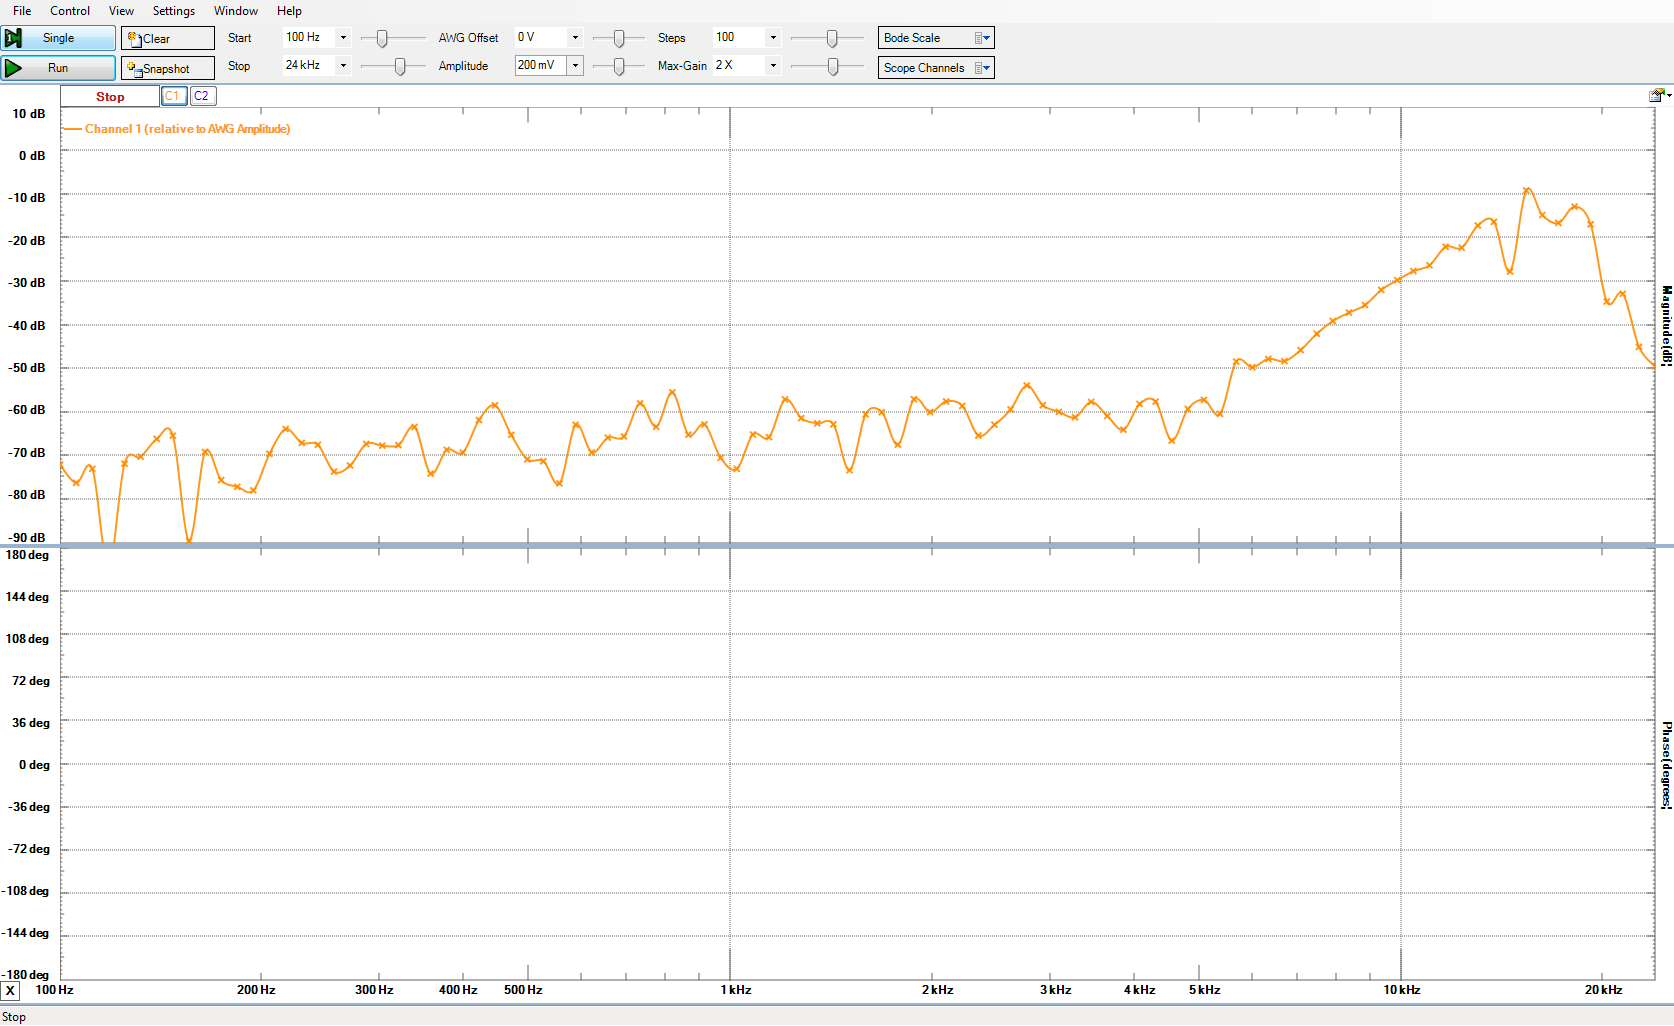
\includegraphics[width=\textwidth]
                  {../presentation/highpass-final.png}
                  \caption{Coefficient Input Process}
                  \label{fig:c1}
\end{figure}
\begin{figure}[!htb]
  \centering
  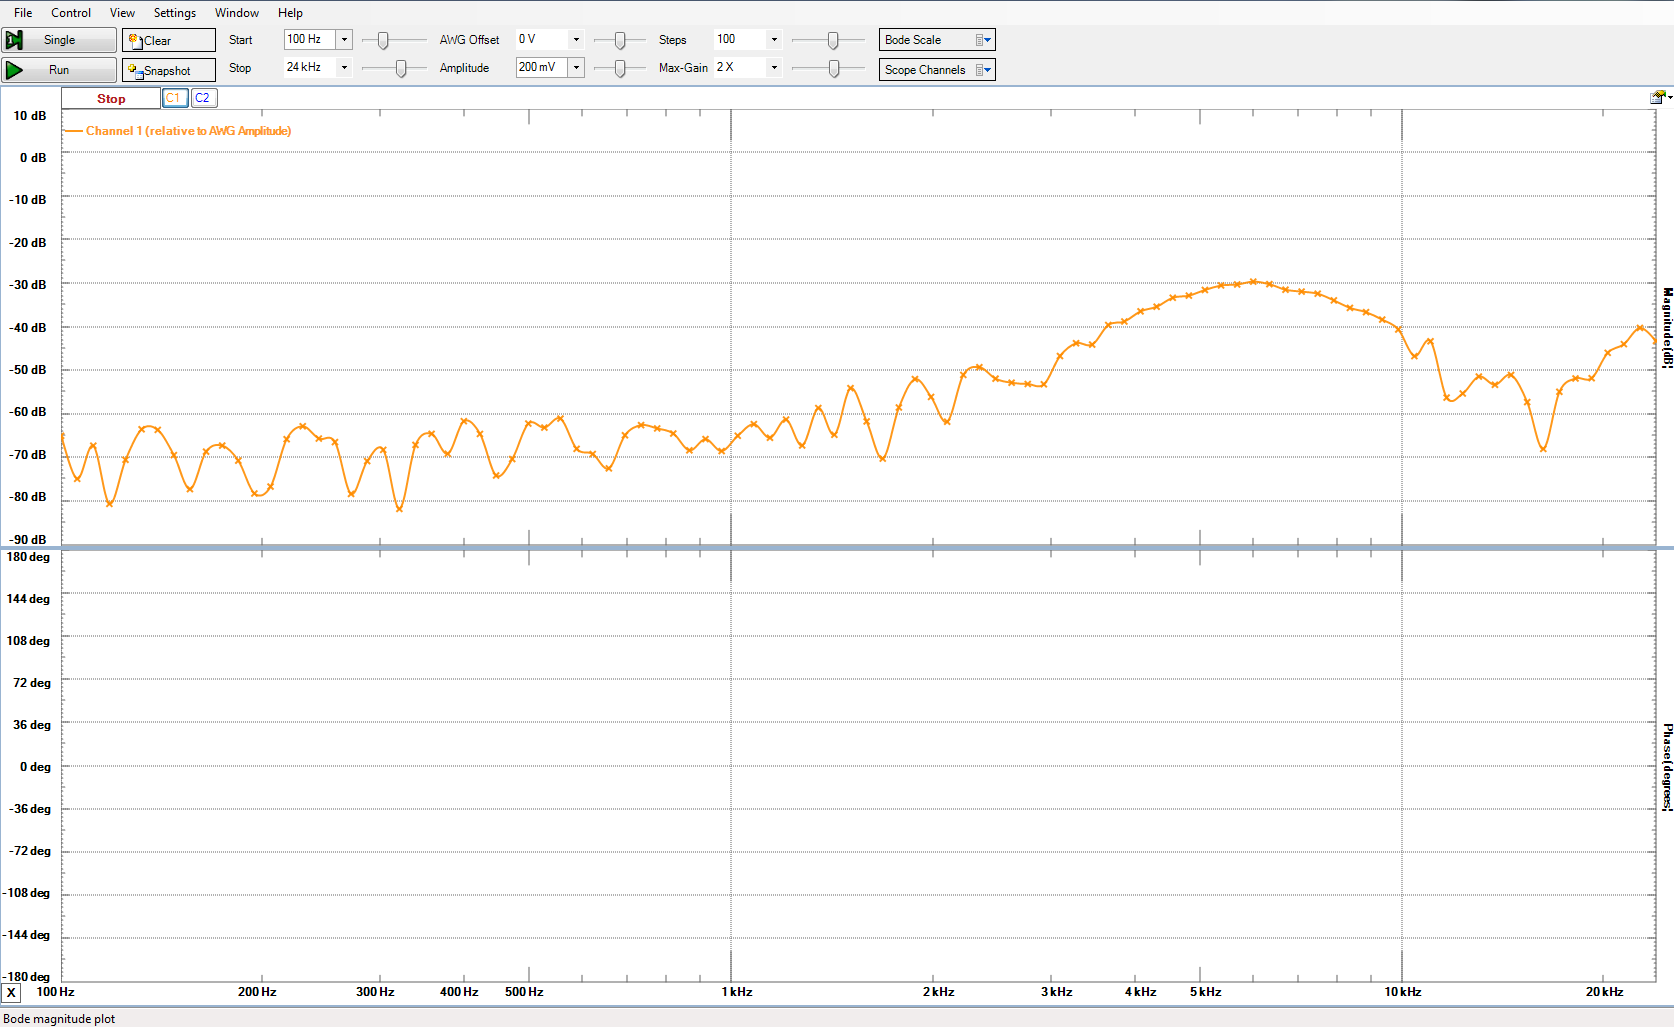
\includegraphics[width=\textwidth]
                  {../presentation/bandpass-final.png}
                  \caption{Coefficient Output Loop}
                  \label{fig:c2}
\end{figure}


%% \printbibliography[
%% heading=bibintoc,
%% title={Resources}
%% ]

\end{document}
